\PassOptionsToPackage{unicode=true}{hyperref} % options for packages loaded elsewhere
\PassOptionsToPackage{hyphens}{url}
%
\documentclass[]{book}
\usepackage{lmodern}
\usepackage{amssymb,amsmath}
\usepackage{ifxetex,ifluatex}
\usepackage{fixltx2e} % provides \textsubscript
\ifnum 0\ifxetex 1\fi\ifluatex 1\fi=0 % if pdftex
  \usepackage[T1]{fontenc}
  \usepackage[utf8]{inputenc}
  \usepackage{textcomp} % provides euro and other symbols
\else % if luatex or xelatex
  \usepackage{unicode-math}
  \defaultfontfeatures{Ligatures=TeX,Scale=MatchLowercase}
\fi
% use upquote if available, for straight quotes in verbatim environments
\IfFileExists{upquote.sty}{\usepackage{upquote}}{}
% use microtype if available
\IfFileExists{microtype.sty}{%
\usepackage[]{microtype}
\UseMicrotypeSet[protrusion]{basicmath} % disable protrusion for tt fonts
}{}
\IfFileExists{parskip.sty}{%
\usepackage{parskip}
}{% else
\setlength{\parindent}{0pt}
\setlength{\parskip}{6pt plus 2pt minus 1pt}
}
\usepackage{hyperref}
\hypersetup{
            pdftitle={MA 5124 Financial Time Series Analysis \& Forecasting},
            pdfauthor={Dr.~Priyanga D. Talagala},
            pdfborder={0 0 0},
            breaklinks=true}
\urlstyle{same}  % don't use monospace font for urls
\usepackage{color}
\usepackage{fancyvrb}
\newcommand{\VerbBar}{|}
\newcommand{\VERB}{\Verb[commandchars=\\\{\}]}
\DefineVerbatimEnvironment{Highlighting}{Verbatim}{commandchars=\\\{\}}
% Add ',fontsize=\small' for more characters per line
\usepackage{framed}
\definecolor{shadecolor}{RGB}{248,248,248}
\newenvironment{Shaded}{\begin{snugshade}}{\end{snugshade}}
\newcommand{\AlertTok}[1]{\textcolor[rgb]{0.94,0.16,0.16}{#1}}
\newcommand{\AnnotationTok}[1]{\textcolor[rgb]{0.56,0.35,0.01}{\textbf{\textit{#1}}}}
\newcommand{\AttributeTok}[1]{\textcolor[rgb]{0.77,0.63,0.00}{#1}}
\newcommand{\BaseNTok}[1]{\textcolor[rgb]{0.00,0.00,0.81}{#1}}
\newcommand{\BuiltInTok}[1]{#1}
\newcommand{\CharTok}[1]{\textcolor[rgb]{0.31,0.60,0.02}{#1}}
\newcommand{\CommentTok}[1]{\textcolor[rgb]{0.56,0.35,0.01}{\textit{#1}}}
\newcommand{\CommentVarTok}[1]{\textcolor[rgb]{0.56,0.35,0.01}{\textbf{\textit{#1}}}}
\newcommand{\ConstantTok}[1]{\textcolor[rgb]{0.00,0.00,0.00}{#1}}
\newcommand{\ControlFlowTok}[1]{\textcolor[rgb]{0.13,0.29,0.53}{\textbf{#1}}}
\newcommand{\DataTypeTok}[1]{\textcolor[rgb]{0.13,0.29,0.53}{#1}}
\newcommand{\DecValTok}[1]{\textcolor[rgb]{0.00,0.00,0.81}{#1}}
\newcommand{\DocumentationTok}[1]{\textcolor[rgb]{0.56,0.35,0.01}{\textbf{\textit{#1}}}}
\newcommand{\ErrorTok}[1]{\textcolor[rgb]{0.64,0.00,0.00}{\textbf{#1}}}
\newcommand{\ExtensionTok}[1]{#1}
\newcommand{\FloatTok}[1]{\textcolor[rgb]{0.00,0.00,0.81}{#1}}
\newcommand{\FunctionTok}[1]{\textcolor[rgb]{0.00,0.00,0.00}{#1}}
\newcommand{\ImportTok}[1]{#1}
\newcommand{\InformationTok}[1]{\textcolor[rgb]{0.56,0.35,0.01}{\textbf{\textit{#1}}}}
\newcommand{\KeywordTok}[1]{\textcolor[rgb]{0.13,0.29,0.53}{\textbf{#1}}}
\newcommand{\NormalTok}[1]{#1}
\newcommand{\OperatorTok}[1]{\textcolor[rgb]{0.81,0.36,0.00}{\textbf{#1}}}
\newcommand{\OtherTok}[1]{\textcolor[rgb]{0.56,0.35,0.01}{#1}}
\newcommand{\PreprocessorTok}[1]{\textcolor[rgb]{0.56,0.35,0.01}{\textit{#1}}}
\newcommand{\RegionMarkerTok}[1]{#1}
\newcommand{\SpecialCharTok}[1]{\textcolor[rgb]{0.00,0.00,0.00}{#1}}
\newcommand{\SpecialStringTok}[1]{\textcolor[rgb]{0.31,0.60,0.02}{#1}}
\newcommand{\StringTok}[1]{\textcolor[rgb]{0.31,0.60,0.02}{#1}}
\newcommand{\VariableTok}[1]{\textcolor[rgb]{0.00,0.00,0.00}{#1}}
\newcommand{\VerbatimStringTok}[1]{\textcolor[rgb]{0.31,0.60,0.02}{#1}}
\newcommand{\WarningTok}[1]{\textcolor[rgb]{0.56,0.35,0.01}{\textbf{\textit{#1}}}}
\usepackage{longtable,booktabs}
% Fix footnotes in tables (requires footnote package)
\IfFileExists{footnote.sty}{\usepackage{footnote}\makesavenoteenv{longtable}}{}
\usepackage{graphicx,grffile}
\makeatletter
\def\maxwidth{\ifdim\Gin@nat@width>\linewidth\linewidth\else\Gin@nat@width\fi}
\def\maxheight{\ifdim\Gin@nat@height>\textheight\textheight\else\Gin@nat@height\fi}
\makeatother
% Scale images if necessary, so that they will not overflow the page
% margins by default, and it is still possible to overwrite the defaults
% using explicit options in \includegraphics[width, height, ...]{}
\setkeys{Gin}{width=\maxwidth,height=\maxheight,keepaspectratio}
\setlength{\emergencystretch}{3em}  % prevent overfull lines
\providecommand{\tightlist}{%
  \setlength{\itemsep}{0pt}\setlength{\parskip}{0pt}}
\setcounter{secnumdepth}{5}
% Redefines (sub)paragraphs to behave more like sections
\ifx\paragraph\undefined\else
\let\oldparagraph\paragraph
\renewcommand{\paragraph}[1]{\oldparagraph{#1}\mbox{}}
\fi
\ifx\subparagraph\undefined\else
\let\oldsubparagraph\subparagraph
\renewcommand{\subparagraph}[1]{\oldsubparagraph{#1}\mbox{}}
\fi

% set default figure placement to htbp
\makeatletter
\def\fps@figure{htbp}
\makeatother

\usepackage{booktabs}
\usepackage{amsthm}
\makeatletter
\def\thm@space@setup{%
  \thm@preskip=8pt plus 2pt minus 4pt
  \thm@postskip=\thm@preskip
}
\makeatother
\usepackage[]{natbib}
\bibliographystyle{apalike}

\title{MA 5124 Financial Time Series Analysis \& Forecasting}
\author{Dr.~Priyanga D. Talagala}
\date{2020-11-02}

\begin{document}
\maketitle

{
\setcounter{tocdepth}{1}
\tableofcontents
}
\hypertarget{course-syllabus}{%
\chapter*{Course Syllabus}\label{course-syllabus}}
\addcontentsline{toc}{chapter}{Course Syllabus}

\pagenumbering{arabic}

\textbf{Module Code:} MA 5124

\textbf{Title:} Financial Time Series Analysis \& Forecasting

\textbf{Credits:} 4

\hypertarget{pre-requiites}{%
\section*{Pre-requiites}\label{pre-requiites}}
\addcontentsline{toc}{section}{Pre-requiites}

None

\hypertarget{learning-objectives}{%
\section*{Learning Objectives}\label{learning-objectives}}
\addcontentsline{toc}{section}{Learning Objectives}

\begin{itemize}
\tightlist
\item
  The purpose of this course is to provide students with introductory tools for the time series analysis of financial time series.
\item
  Analyze of data series based on stochastic and non stochastic models
\end{itemize}

\hypertarget{learning-outcomes}{%
\section*{Learning Outcomes}\label{learning-outcomes}}
\addcontentsline{toc}{section}{Learning Outcomes}

\begin{itemize}
\tightlist
\item
  On successful completion of this course, students will be able to provide more than an introductory treatment of the topics.
\item
  Students are encouraged to pursue further study in this area if they find that the topics covered in this course.
\end{itemize}

\hypertarget{outline-syllabus}{%
\section*{Outline Syllabus}\label{outline-syllabus}}
\addcontentsline{toc}{section}{Outline Syllabus}

\begin{itemize}
\tightlist
\item
  Definition and examples of time series
\item
  back-shift and differencing-operators, - strong and weak stationarity, definition of ACF, PACF.
\item
  Definitions and properties of the \(MA(q), MA(\infty), AR(p), AR(\infty)\)
  and \(ARMA(p,q)\),in particualr their acf's
\item
  causal stationarity of AR
\item
  invertibility of MA models and causal stationarity and invertibility of ARMA; - concept of spectral density function and its applications
\item
  definition and properties of integrated \(ARIMA(p,d,q)\) processes
\item
  definition and properties of random walks with or without drift.
\item
  Model selection following the AIC and BIC
\item
  brief introduction to linear prediction and calculation of forecasting intervals for normal ARMA models
\item
  point and interval forecasts for normal random walks with or without drift.
\item
  Definition and properties of the VAR (vector autoregressive) model, arrange a univariate time series as a multivariate Markov model.
\item
  Nonlinear properties of financial time series
\item
  definition and properties of the well known ARCH, GARCH etc.
\item
  Cointegration in Single Equations, Modeling and Forecasting Financial Time Series.
\end{itemize}

\hypertarget{method-of-assessment}{%
\section*{Method of Assessment}\label{method-of-assessment}}
\addcontentsline{toc}{section}{Method of Assessment}

\begin{itemize}
\tightlist
\item
  Assignment 30\%
\item
  End-semester examination 70\%
\end{itemize}

\hypertarget{lecturer}{%
\section*{Lecturer}\label{lecturer}}
\addcontentsline{toc}{section}{Lecturer}

Dr.~Priyanga D. Talagala

\hypertarget{schedule}{%
\section*{Schedule}\label{schedule}}
\addcontentsline{toc}{section}{Schedule}

Lectures:

\begin{itemize}
\tightlist
\item
  Sunday {[}9.00am -12.00 noon{]}
\end{itemize}

\hypertarget{copyright-notice}{%
\section*{Copyright Notice}\label{copyright-notice}}
\addcontentsline{toc}{section}{Copyright Notice}

My lectures and course materials, including presentations, tests, exams, outlines, and similar materials, are protected by copyright. I am the exclusive owner of copyright in those materials I create. I encourage you to take notes and make copies of course materials for your own educational use. However, you may not, nor may you knowingly allow others to reproduce or distribute lecture notes and course materials publicly without my express written consent.

\hypertarget{intro}{%
\chapter{Introduction}\label{intro}}

You can label chapter and section titles using \texttt{\{\#label\}} after them, e.g., we can reference Chapter \ref{intro}. If you do not manually label them, there will be automatic labels anyway, e.g., Chapter \ref{methods}.

Figures and tables with captions will be placed in \texttt{figure} and \texttt{table} environments, respectively.

\begin{Shaded}
\begin{Highlighting}[]
\KeywordTok{par}\NormalTok{(}\DataTypeTok{mar =} \KeywordTok{c}\NormalTok{(}\DecValTok{4}\NormalTok{, }\DecValTok{4}\NormalTok{, }\FloatTok{.1}\NormalTok{, }\FloatTok{.1}\NormalTok{))}
\KeywordTok{plot}\NormalTok{(pressure, }\DataTypeTok{type =} \StringTok{'b'}\NormalTok{, }\DataTypeTok{pch =} \DecValTok{19}\NormalTok{)}
\end{Highlighting}
\end{Shaded}

\begin{figure}

{\centering 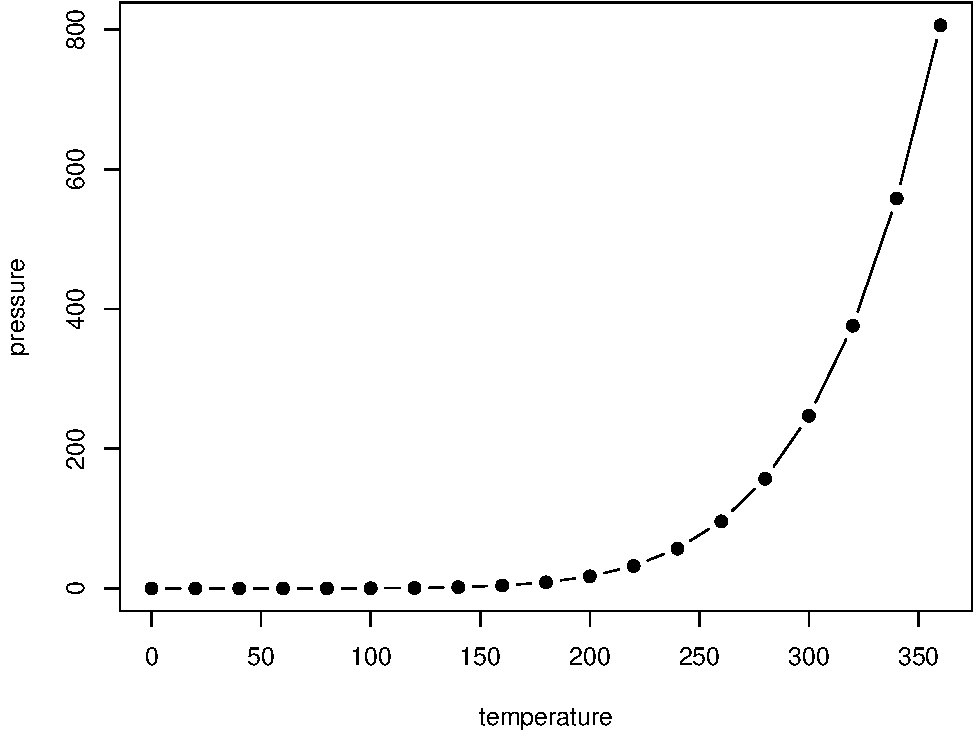
\includegraphics[width=0.8\linewidth]{bookdown-demo_files/figure-latex/nice-fig-1} 

}

\caption{Here is a nice figure!}\label{fig:nice-fig}
\end{figure}

Reference a figure by its code chunk label with the \texttt{fig:} prefix, e.g., see Figure \ref{fig:nice-fig}. Similarly, you can reference tables generated from \texttt{knitr::kable()}, e.g., see Table \ref{tab:nice-tab}.

\begin{Shaded}
\begin{Highlighting}[]
\NormalTok{knitr}\OperatorTok{::}\KeywordTok{kable}\NormalTok{(}
  \KeywordTok{head}\NormalTok{(iris, }\DecValTok{20}\NormalTok{), }\DataTypeTok{caption =} \StringTok{'Here is a nice table!'}\NormalTok{,}
  \DataTypeTok{booktabs =} \OtherTok{TRUE}
\NormalTok{)}
\end{Highlighting}
\end{Shaded}

\begin{table}

\caption{\label{tab:nice-tab}Here is a nice table!}
\centering
\begin{tabular}[t]{rrrrl}
\toprule
Sepal.Length & Sepal.Width & Petal.Length & Petal.Width & Species\\
\midrule
5.1 & 3.5 & 1.4 & 0.2 & setosa\\
4.9 & 3.0 & 1.4 & 0.2 & setosa\\
4.7 & 3.2 & 1.3 & 0.2 & setosa\\
4.6 & 3.1 & 1.5 & 0.2 & setosa\\
5.0 & 3.6 & 1.4 & 0.2 & setosa\\
\addlinespace
5.4 & 3.9 & 1.7 & 0.4 & setosa\\
4.6 & 3.4 & 1.4 & 0.3 & setosa\\
5.0 & 3.4 & 1.5 & 0.2 & setosa\\
4.4 & 2.9 & 1.4 & 0.2 & setosa\\
4.9 & 3.1 & 1.5 & 0.1 & setosa\\
\addlinespace
5.4 & 3.7 & 1.5 & 0.2 & setosa\\
4.8 & 3.4 & 1.6 & 0.2 & setosa\\
4.8 & 3.0 & 1.4 & 0.1 & setosa\\
4.3 & 3.0 & 1.1 & 0.1 & setosa\\
5.8 & 4.0 & 1.2 & 0.2 & setosa\\
\addlinespace
5.7 & 4.4 & 1.5 & 0.4 & setosa\\
5.4 & 3.9 & 1.3 & 0.4 & setosa\\
5.1 & 3.5 & 1.4 & 0.3 & setosa\\
5.7 & 3.8 & 1.7 & 0.3 & setosa\\
5.1 & 3.8 & 1.5 & 0.3 & setosa\\
\bottomrule
\end{tabular}
\end{table}

You can write citations, too. For example, we are using the \textbf{bookdown} package \citep{R-bookdown} in this sample book, which was built on top of R Markdown and \textbf{knitr} \citep{xie2015}.

\hypertarget{literature}{%
\chapter{Literature}\label{literature}}

Here is a review of existing methods.

\hypertarget{methods}{%
\chapter{Methods}\label{methods}}

We describe our methods in this chapter.

\hypertarget{applications}{%
\chapter{Applications}\label{applications}}

Some \emph{significant} applications are demonstrated in this chapter.

\hypertarget{example-one}{%
\section{Example one}\label{example-one}}

\hypertarget{example-two}{%
\section{Example two}\label{example-two}}

\hypertarget{final-words}{%
\chapter{Final Words}\label{final-words}}

We have finished a nice book.

\bibliography{book.bib,packages.bib}

\end{document}
